\section{Week 5: 9th - 15th February 2026}

\subsection{Tuesday 10th February}

\subsubsection{Meeting 5: Zhaoting and Alkistis (Zoom)}

\begin{itemize}
    \item We just went over the code snippets I was emailed last.
    \item I think I probably misunderstood what I was meant to do or didn't put enough thought into the code because I don't think I fully understood the graphs I was plotting.
    \item I didn't plot the right thing for the second plot of each of the cylindrical power spectrum graphs. I need to have another look at the code and fix it. I don't fully understand what I didn't plot correctly but I will have another look at the code.
    \item It was something to do with the fact that I need to plot the residuals of the whole signal and but just part of it so the ratio is also off.
    \item In my description of Figure 26, I originally stated that the first 2 modes and very smooth and linear. Linear is not a correctly description. The spectral index graph is not linear but it is smooth. And since the graph only covers a small frequency range, it appears linear.
    \item I also asked why the first two modes are smooth and the others are not. This does not really matter. It is just the eigenvalues and the first 3 modes that matter. Plotting the eigenvectors just show us what the signal looks like at those modes.
    \item The noise power spectrum is as expected. It is completely uniform. It is a component that is easy to just put in and therefore easy to remove.
    \item It is just that the first 3 modes are the largest. The rest of the modes are of similar size. This is highlighted by the log plot.
    \item To-do now:
    \begin{itemize}
        \item Fix the cylindrical power spectrum graphs
        \item Look at GPR notebook. Zhaoting said it was not fully finished and polished but it should be good to get some experience in finishing and running code myself.
        \item Look at eigenvectors plot from paper Alkistis sent. See Figure 27.
    \end{itemize}
\end{itemize}
    
% source: https://arxiv.org/abs/1504.07527
        \begin{figure}
            \centering
            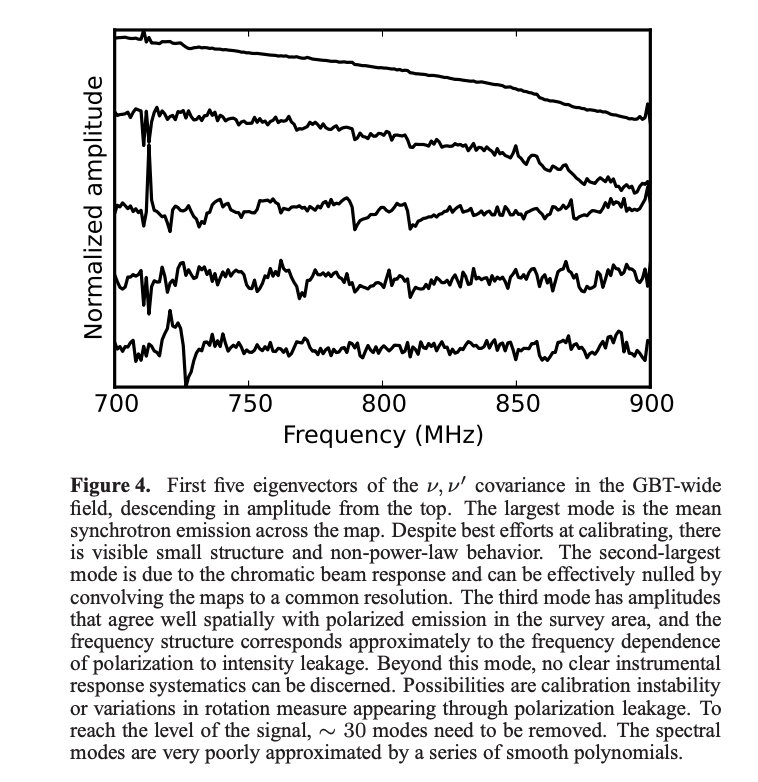
\includegraphics[width=0.5\linewidth]{image.png}
            \caption{Eigenvectors plot from a real data analysis paper}
            \label{fig:placeholder}
        \end{figure}